\begin{figure}
  \centering
    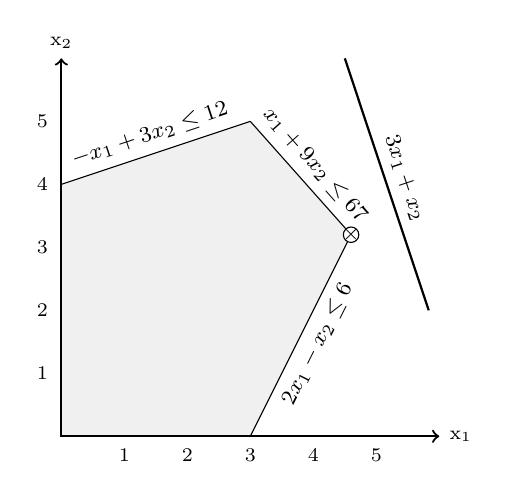
\begin{tikzpicture}[scale=0.8,font=\scriptsize]

      \fill[fill={rgb:black,1;white,16}] (0,0) -- (0,4) -- (3,5) -- (4.6,3.2) -- (3,0) -- cycle;
      \draw [<->,thick] (0,6) node (yaxis) [above] {\sansitalicfont
      x\textsubscript{2}}
        |- (6,0) node (xaxis) [right] {\sansitalicfont x\textsubscript{1}};

      \foreach \x in {1,...,5} \node at (\x,-0.3) {\sansfont \x};
      \foreach \y in {1,...,5} \node at (-0.3, \y) {\sansfont \y};

      \draw (0, 4) -- node[above, sloped] {\footnotesize $-x_1 + 3x_2 \leq 12$} (3,5);
      \draw (3, 0) -- node[below, sloped] {\footnotesize $2x_1 - x_2 \leq 6$}
      (4.6,3.2);
      \draw (3, 5) -- node[above, sloped] {\footnotesize $x_1 + 9x_2 \leq 67$}
      (4.6,3.2);
      
      \draw [thick] (4.5,6) -- node[above, sloped] {\footnotesize $3x_1 + x_2$}
      (5.833,2); 
     
      \draw (4.6,3.2) node[circle,fill=white, inner sep=-0.9pt, draw=black, line 
      width=0.4pt] {\scriptsize$\times$};
    \end{tikzpicture}
 \caption{Graphical representation of a typical LP problem}\label{fig:lpplot1}
 \end{figure}
